\documentclass[11pt,a4paper]{report}
\usepackage[utf8]{inputenc}
\usepackage[french]{babel}
\usepackage[T1]{fontenc}
\usepackage{amsmath}
\usepackage{amsfonts}
\usepackage{amssymb}
\usepackage{xcolor}
\usepackage{gensymb}

\usepackage{geometry}
\geometry{hmargin=2.5cm,vmargin=1.5cm}
\usepackage{wasysym}
\usepackage{graphicx}

\author{Mathieu Sarrat}
\title{LC7 - Cinétique et catalyse}

\makeatletter
\renewcommand{\thesection}{\@arabic\c@section}
\makeatother

\begin{document}
\maketitle

\section*{Pré-requis, niveau, objectifs}

\subsubsection*{Niveau}
\begin{itemize}
	\item Terminale S
\end{itemize}

\subsubsection*{Pré-Requis}
\begin{itemize}
	\item Oxydoréduction.
	\item Spectrophotométrie UV-Visible et conductimétrie.
	\item Tableau d'avancement
	\item Réactions de combustion.
\end{itemize}

\subsubsection*{Objectifs}
\begin{itemize}
	\item Introduire l'aspect cinétique d'une réaction chimique et son importance pratique.
	\item Définir les principaux facteurs agissant sur la vitesse d'une réaction.
	\item Connaître les grands types de catalyse et quelques grandes applications.
\end{itemize}

\newpage
\section*{Introduction}

Jusqu'à présent, nous n'avons écrit que des équations bilan pour modéliser les réactions chimiques. Celles-ci nous renseignent sur les réactifs consommés et les produits formés, mais ne donnent aucune information quant à la rapidité de la transformation chimique qui se déroule. Le facteur temps est absent de la modélisation.\\

La cinétique chimique étudie l'évolution temporelle des systèmes chimiques. Cette discipline a une grande importance dans le milieu industriel, où l'on souhaite produire beaucoup en un minimum de temps.

\begin{itemize}
	\item certaines réactions chimiques paraissent immédiates, c'est le cas d'un grand nombre de réactions de dosage, que l'on souhaite rapides pour des raisons pratiques évidentes \textcolor{red}{(Manip : verser des ions permanganate dans une solution d'ions $\text{Fe}^{2+}$, la couleur fuschia disparaît instantanément.)};\\
	
	\item plus lente (quelques minutes) \textcolor{red}{(Manip : faire réagir l'eau oxygénée avec 	les ions iodure et constater l'apparition d'une couleur orange, lentement, témoignant de la présence de diiode)};\\
	
	\item très lentes, des jours ou des années, comme la formation de la rouille.\\
\end{itemize}

Comment modéliser l'évolution temporelle d'une réaction chimique ? Peut-on influer sur cette évolution pour accélérer une réaction désirée, ou ralentir voire bloquer une réaction indésirable ? Nous allons répondre à ces deux questions durant cette leçon.

\section{Évolution temporelle d'un système chimique}

\subsection{Modélisation}

Pour caractériser l'évolution d'un système chimique, on peut adopter plusieurs approches :
\begin{itemize}
	\item suivre la diminution de la quantité de matière d'un réactif au cours du temps, 
	\item suivre l'augmentation de la quantité de matière d'un produit au cours du temps,
	\item suivre l'avancement de la réaction au cours du temps.\\
\end{itemize}

Reprenons le cas de la réaction des ions iodure avec l'eau oxygénée, que l'on peut supposer totale ($E\degree(\text{I}^2/\text{I}^-) = 0.54$ V et $E\degree(\text{H}_2\text{O}_{2}/\text{H}_2\text{O}) = 1.78$) :
\begin{equation}
 	\boxed{\text{H}_2\text{O}_{2,\text{(aq)}} + 2 \text{I}^{-}_\text{(aq)} + 2 \text{H}^+_			\text{(aq)} = I_{2,\text{(aq)}} + 2\text{H}_2\text{O}_\text{(l)}}\\
\end{equation}

\textbf{Dresser le tableau d'avancement, en concentrations :}
\begin{equation}
	n_{\text{H}_2\text{O}_2} = n_0 - x,
\end{equation}
\begin{equation}
	n_{\text{I}^-} = n_1 - 2x,
\end{equation}
\begin{equation}
 	n_{\text{I}_2} = x.
\end{equation}

On voit que \textbf{connaître la quantité de matière d'une seule espèce permet de déterminer l'avancement} pourvu que l'on connaisse la composition initiale, et donc la quantité de matière de toutes les autres espèces ayant réagi. Suivre l'avancement en fonction du temps nous permet donc de connaître à tout instant la composition du milieu réactionnel.

\newpage
\subsection{Méthode de suivi de l'avancement}

Concrètement, comment va-t-on faire pour suivre cinétiquement une réaction ?\\

\begin{itemize}
	\item Un \textbf{suivi qualitatif} est possible, lorsqu'au cours de la réaction on détecte 		un dégagement gazeux, un changement de couleur, la formation ou la disparition d'un solide : en d'autres termes, en phénomène flagrant, bien repérable. Cela permet de savoir à vue d'œil quand la réaction est terminée.\\
	
	\item \textbf{Quantitativement}, on doit mesurer une grandeur physique reliée à l'avancement réactionnel. Par exemple :
	\begin{itemize}
		\item la conductivité, par conductimétrie si des ions sont formés ou sont consommés,
		\item l'absorbance, par spectroscopie UV-visible, si des espèces absorbant dans le 					visible (colorées) ou dans le proche UV sont consommées ou produites.\\
	\end{itemize}
	
	\item \textbf{Manip : suivi spectrophotométrique de la formation du diiode} :
	\begin{itemize}
		\item \textbf{Protocole :} Le Maréchal, Chimie Générale, p271. 
		Mettre 8 mL de KI au lieu de 5 mL de KI et 3 d'eau.
		\item Que faire concrètement le jour J : courbe en préparation, exploitation en direct. 			Relancer la manip en direct (avec une autre température, si possible), si acquisition 				automatique possible et supposer l'état final connu pour relever le temps de demi-réaction.
		\item Doser la solution d'eau oxygénée pour prédire la valeur finale de l'absorbance.\\
	\end{itemize}

	\item \textbf{Exploitation :} des résultats faits en préparation.
	\begin{itemize}
		\item La seule espèce colorée, de couleur jaune orangée est le diiode. La solution aqueuse 			va absorber dans le visible. On utilise la loi de Beer-Lambert pour relier la quantité de 			diiode à la valeur de l'absorbance :
		\begin{equation}
			A_\lambda(t) = k_\lambda [\text{I}_2](t) = \frac{k_\lambda}{V} n_{\text{I}_2}(t) .
		\end{equation}
		L'évolution de $A_\lambda$ est donc représentative de celle de la concentration en diiode. 			La valeur de $k$ dépend du réglage du spectrophotomètre.\\
	\end{itemize}
\end{itemize}

\textbf{Remarque : ce n'est pas le diiode mais l'ion triiodure} que l'on retrouve réellement dans la solution. Il y a donc un coefficient 3 au lieu de 2 devant l'iodure dans l'équation bilan. Si on suit les quantités indiquées dans le protocole, on est certain que le peroxyde d'hydrogène sera le réactif limitant, ce qui ne change rien à la manip. 

\subsection{Temps de demi-réaction}

\begin{itemize}
	\item \textbf{Définition :} le temps de demi-réaction $t_{1/2}$ est la durée au bout de 			laquelle l'\textbf{avancement réactionnel atteint la moitié de sa valeur finale}. Il s'exprime 		en secondes, minutes, heures ... selon le cas. Il constitue une durée caractéristique de la 		réaction chimique.\\
	
	\item Insistons bien sur un point : si $t = 2t_{1/2}$, la réaction n'est pas finie, car 			l'évolution des quantités de matière n'est pas linéaire dans le temps.\\
	
	\item \textcolor{red}{Détermination du temps de demi-réaction pour la réaction de formation de 		$\text{I}_{\text{2}}$ à partir des données expérimentales}.
\end{itemize}

\newpage
\section{Facteurs cinétiques}

Nous venons de voir comment caractériser, de façon simplifiée, la rapidité d'une réaction chimique. Survient une nouvelle question : une réaction est-elle rapide ou lente par essence ? La réponse est non : cela dépend de nombreux facteurs.

Parmi ces facteurs, nous mettrons en évidence les trois principaux :
\begin{itemize}
	\item température,
	\item concentration des réactifs,
	\item présence d'un catalyseur.\\
\end{itemize}

\textbf{Remarque :} la nature du solvant (notamment pour les substitutions nucléophiles), la lumière, l'état de surface des réactifs s'ils sont solides (broyés ou non, surface oxydée ou non), voire l'éclairement peuvent également jouer.

\subsection{Effet de la concentration}

\begin{itemize}
	\item \textbf{Manip : Décomposition des ions thiosulfate en milieu acide (Sarrazin Verdaguer 		p183)}.
		\begin{itemize}
			\item Bécher 1 : 30 mL d'eau, 20 mL de thiosulfate et 5 mL d'acide,
			\item Bécher 2 : 10 mL d'eau, 40 mL de thiosulfate et 5 mL d'acide.			
		\end{itemize}	
		Ici, l'acide est réactif limitant. Chronométrer ou pas, selon le temps. Eventuellement 				flexcam avec les croix au velleda.\\	 
	
	\item Interprétation : augmenter la concentration d'un réactif accélère la réaction.
	\item \textcolor{red}{Jeter le milieu réactionnel le plus rapide dans un bécher poubelle 			contenant de l'eau et quelques pastilles de soude, pour dégrader le dioxyde de soufre toxique 		libéré par la réaction.}
	
	\item Diluer ralentit la réaction. Ainsi, un ajout soudain d'eau glacée au milieu réactionnel 		produit une trempe conjuguant les deux effets mentionnés : on dilue et on refroidit, ce qui 		ralentit très fortement la réaction. 	
\end{itemize}
\subsection{Effet de la température}

\begin{itemize}
	\item \textbf{Effet de la température :} si la température augmente, la durée de la 			réaction est réduite. Au contraire, si on refroidit, on freine la réaction. Un refroidissement brutal peut même bloquer la réaction (on parle de trempe). La trempe permet de mesurer l'avancement à un instant donné (celui où on a trempé l'échantillon du milieu réactif) : on peut doser le produit sans que les concentrations soient faussées par la réaction.\\
	
	\item \textbf{Décomposition des ions thiosulfate en milieu acide (Sarrazin Verdaguer p183)} :
	\begin{equation}
		\boxed{\text{S}_2\text{O}_3^{2-} + 2\text{H}^+ 
		= \text{SO}_{2,\text{(g)}} + \text{S}_\text{(s)} + \text{H}_2\text{O}_\text{(l)}}
	\end{equation}
	
	Récupérer la solution la moins concentrée de la manip précédente, la diviser dans deux tubes à 	essais : plonger le premier tube dans un bécher contenant de l'eau glacée, plonger le second dans 	un bécher contenant de l'eau chaude (50$\degree$C au robinet).
\end{itemize}

\subsection{Présence d'un catalyseur}

\subsubsection*{a/ Définition et intérêt :} un catalyseur est une \textbf{espèce chimique} différente des réactifs, dont la présence \textbf{diminue la durée de la réaction chimique}. Il réagit avec les réactifs mais est intégralement \textbf{régénéré en fin de réaction}. Il \textbf{n'apparaît donc pas dans l'équation bilan} et est réutilisable.\\

La catalyse ne peut accélérer qu'une réaction thermodynamiquement possible (c'est à dire réalisable sans le catalyseur, même si elle est très lente). Si la réaction est thermodynamique impossible, ajouter un catalyseur ne fera pas démarrer la réaction. Le catalyseur ne modifie que le "chemin réactionnel", c'est à dire les processus microscopiques ayant lieu lors des étapes de la réaction.
			
\subsubsection*{b/ Intérêt :} un très grand nombre de réactions biochimiques sont catalysées, 		par exemple dans le système digestif pour dégrader les aliments ingérés.\\
 	
	Dans l'industrie on les utilise pour accroître la productivité : la synthèse de l'ammoniac 		(utilisé dans les engrais, entre autres) serait impossible à échelle industrielle sans catalyseur, car la réaction est très lente. On utilise un catalyseur à base de fer (voir procédé Haber en annexe). En chimie organique, utilisation du Nickel (Paul Sabatier) pour catalyser les réactions d'hydrogénation.\\
	
	Le recours à la catalyse est l'un des \textbf{douze piliers de la chimie durable} : on utilise moins d'énergie pour faire une réaction, on réduit le nombre d'étapes (et donc le nombre de déchets et la quantité de solvant).

\subsubsection*{c/ Différents types de catalyse :} 

	\begin{itemize}
	\item \textbf{homogène} : catalyseur et réactifs forment un mélange homogène (même phase, par exemple en solution). Les principaux catalyseurs sont $\text{H}^+$ et les ions métalliques. Pour mettre en évidence l'effet d'un catalyseur sur une réaction, intéressons nous à la décomposition de l'eau oxygénée.
	
	Le peroxyde d'hydrogène appartient à deux couples rédox : $\text{H}_2\text{O}_2/\text{H}_2\text{O}$ où il joue le rôle d'oxydant et $\text{O}_2/\text{H}_2\text{O}_2$ où il joue le rôle de réducteur. L'eau oxygénée ne peut donc pas être stable : elle va se dismuter, selon la réaction
	\begin{equation}
		2\text{H}_2\text{O}_{2,\text{(aq)}} 
		= 2\text{H}_2\text{O}_\text{(l)} + \text{O}_{2,\text{(g)}}
	\end{equation}
	Cette réaction est très lente, mais peut être accélérée par catalyse homogène. 
	\textcolor{red}{Manip : p280 Hatier Terminale S, décomposition du péroxyde d'hydrogène 					catalysée par $\text{Fe}^{3+}$} ou Iodure et péroxodisulfate p 184 du Sarrazin Verdaguer;\\

	\textbf{Protocole :} prendre 3 tubes à essais. 
	\begin{itemize}
		\item Tubes 1 et 2 : 2 mL d'eau oxygénée à 20 volumes. Tube 3 : mettre 2 mL d'eau distillée.
		\item Tube 1 : cinq gouttes de chlorure de sodium. Tubes 2 et 3 : cinq gouttes de chlorure 					de fer III.
	\end{itemize}
	Le premier tube sert de témoin : il contient les ions chlorure et de l'eau oxygénée, mais pas 	les ions ferriques et il ne se passe rien. Les ions chlorure n'ont pas d'effet visible sur la 		décomposition de l'eau oxygénée. Cette dernière a lieu, mais lentement. Le tube 3 ne contient pas d'eau oxygénée mais contient les ions 	ferriques et les ions chlorure, il ne se passe rien. Le second tube contient l'eau oxygénée et les ions ferriques. Un dégagement gazeux est observé (test à l'allumette pour confirmer que du dioxygène est dégagé) : la présence des ions ferriques 		accélère la réaction de décomposition.\\  
		
	\item \textbf{hétérogène} : catalyseur et réactifs forment un mélange hétérogène (phases 		différentes). Les catalyseurs sont généralement des solides : métaux (platine) ou oxydes 		métalliques. Le pot catalytique;\\
	
	Les moteurs à essence rejettent des gaz polluants, résultant du non respect des proportions 	stoechiométriques lors de la combustion des hydrocarbures par le dioxygène : du monoxyde de carbone, des hydrocarbures non brûlés et des oxydes d'azote (\text{NO} et $\text{NO}_2$) sont émis par le moteur. Le pot catalytique a pour objectif de dégrader ces gaz (environ 95\%). Un pot catalytique est constitué d'un isolant thermique en céramique creusé en nid d'abeille, la paroi des alvéoles étant imprégnée de métaux comme le platine (Pt), le rhodium (Rh) et le palladium (Pd). Ces métaux agissent comme catalyseurs dans :
	\begin{itemize}
		\item l'oxydation du monoxyde de carbone en dioxyde de carbone,
		\item la réduction des oxydes d'azote en diazote,
		\item l'oxydation en eau et dioxyde de carbone des hydrocarbures non brûlés par le 						moteur.\\
	\end{itemize}
	\textbf{Remarque :} essence sans plomb nécessaire, car le plomb recouvre les métaux qui ne 		peuvent plus catalyser les réactions. Elles deviennent lentes ou peuvent même être bloquées.\\
	
	\item \textbf{enzymatique} : le catalyseur est une protéine, appelée enzyme. Les enzymes présentent des cavités ayant une structure spatiale telle que seuls certains réactifs, de forment adaptée, peuvent s'y fixer, un peu comme une clé dans une serrure. La catalyse enzymatique a une  très grande importance en biochimie, et en particulier dans le mécanisme de la digestion des aliments.\\ 
	
	La digestion est un ensemble de processus mécaniques et chimiques permettant à un organisme 	vivant (nous) de transformer par réaction chimique les aliments consommés (eux) en nutriments assimilables. Divers types de sécrétions digestives (salive, sucs gastrique, pancréatique, intestinal et bile) sont produits par divers organes pour faciliter la digestion. Ces sécrétions contiennent des enzymes chargées de favoriser les réactions chimiques produisant des acides aminés, acides gras, vitamines ... à partir des protides, lipides et glucides (p 296 Physique Chimie Terminale S, Hatier (Nouveau Microméga)).\\
	
	Elles sont particulièrement efficaces : pour briser les liaisons chimiques au sein des protéines sans enzymes, on doit avoir recours à une catalyse par les ions $H^+$ de concentration 6 mol/L à chaud (110$\degree$C), pendant 24 heures environ, là où la digestion ne dure que quelques heures chez l'être humain.
\end{itemize}

\section*{Conclusion}

Il est possible de suivre dans le temps l'avancement d'une réaction, par des méthodes physiques (mesure de la conductivité, de l'absorbance) ou chimiques (par trempe puis dosage). Le temps de demi-réaction est une grandeur nous permettant d'évaluer la rapidité d'une réaction chimique.\\

Nous avons également vu qu'il était possible de modifier la vitesse d'une réaction, en agissant sur des facteurs comme la température, la concentration en réactifs ou en introduisant un catalyseur dans le milieu. Ces derniers sont des espèces chimiques régénérées en fin de réaction, permettant d'accélérer une réaction qui est thermodynamiquement possible. La catalyse est appelée à jouer un rôle de plus en plus important en chimie (économies d'énergie, de réactifs) et est un ingrédient majeur dans la compréhension de mécanismes biologiques.

\newpage
\section*{Annexes}

\subsection*{Synthèse de l'ammoniac}

\textbf{Procédé Haber} : hydrogénation du diazote atmosphérique en présence d'un catalyseur (fer et potasse).
\begin{equation}
	\text{N}_{2,(g)} + 3\;\text{H}_{2,(g)}  \rightleftarrows 2\;\text{NH}_{3,(g)} 
\end{equation}
Pour déplacer l'équilibre vers la droite :
\begin{itemize}
	\item augmenter la pression (loi de le Châtelier, une augmentation de la pression déplace l'équilibre dans le sens de la diminution du nombre total de moles de gaz);
	\item maintenir une température faible (loi de Van't Hoff, une augmentation de $T$ déplace l'équilibre vers le sens endothermique, la réaction étant exothermique on doit diminuer $T$);
\end{itemize}
En pratique, la réaction est très lente à basse température (cinétique). Elle se fait donc à une température plus élevée (environ 450$\degree$C) qui permet d'obtenir une quantité appréciable d'ammoniac dans un temps satisfaisant.

\subsection*{Mécanisme probable de formation de la rouille}

Quand le fer entre en contact avec l'eau, un processus électrochimique lent commence, dont les étapes pourraient (c'est apparemment encore une question ouverte) être :\\
\begin{itemize}
	\item \textbf{Etape 1 : oxydation du fer et réduction du dioxygène}
	\begin{equation}
		\text{Fe} + 2\text{OH}^- \rightarrow \text{Fe(OH)}_2 + 2\text{e}^-
	\end{equation}
	\begin{equation}
		2\text{H}_2\text{O} + \text{O}_2 + 4 \text{e}^- \rightarrow 4\text{OH}^-. 
	\end{equation}
	
	\item \textbf{Etape 2 : oxydation de l'hydroxyde de fer(II) en hydroxyde de fer(III)}
	\begin{equation}
		4\text{Fe(OH)}_2 + 2\text{H}_2\text{O} + \text{O}_2\rightarrow 4\text{Fe(OH)}_3 
	\end{equation}	 
	\item \textbf{Etape 3 : formation de l'oxyde de fer(III) hydraté}
	\begin{equation}
		2\text{Fe(OH)}_3 \rightarrow \text{Fe}_2\text{O}_3 + 3\text{H}_2\text{O}.
	\end{equation}
\end{itemize}

\newpage
\subsection*{Triglyrécides, acides aminés, protéines, glucose}

\subsubsection*{Glycérol et triglycérides}
\begin{figure}[h!]
	\begin{center}
		\begin{tabular}{cc}
  		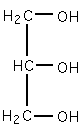
\includegraphics[scale = 1]{glycerol.png} &
   		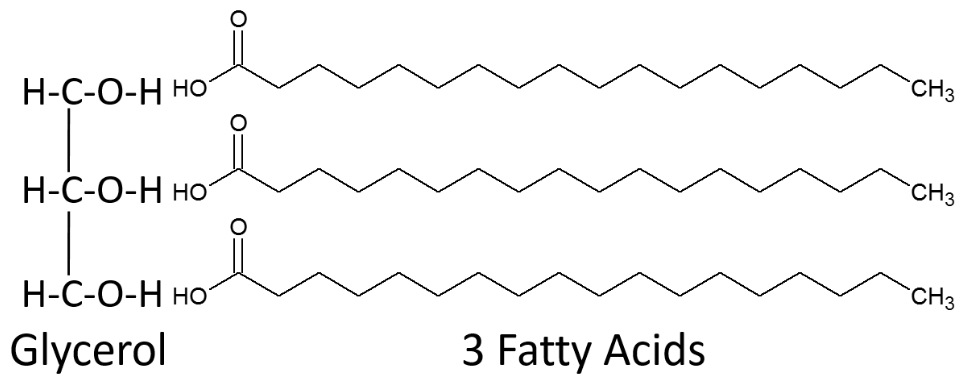
\includegraphics[scale = 0.4]{triglycerides.png}\\
	\end{tabular}
	\caption{Gauche : glycérol. Droite : un triglycéride.}
	\end{center}
\end{figure}

\subsubsection*{Acides alpha-aminés}

\begin{figure}[h!]
	\begin{center}
		\begin{tabular}{cc}
  		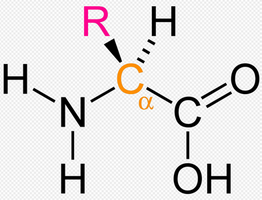
\includegraphics[scale = 0.5]{alpha_amine.png} &
   		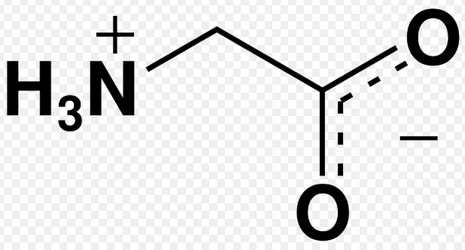
\includegraphics[scale = 0.35]{glycine.png}\\
	\end{tabular}
	\caption{Gauche : forme générale d'un acide $\alpha-$aminé. Droite : la glycine est le plus 			simple d'entre eux, représentée ici sous forme de zwitterion.}
	\end{center}
\end{figure}

Le groupe carboxyle $-\text{COOH}$ est un acide faible, ce qui signifie qu'il tend à libérer un proton pour donner un carboxylate $-\text{COO}^-$ chargé négativement. La forme carboxylate est prédominante à pH supérieur au pKa de l'acide carboxylique, c'est-à-dire environ 2,2 pour les acides aminés protéinogènes. De façon symétrique, le groupe amine $-\text{NH}_2$ est une base faible, ce qui signifie qu'il tend à recevoir un proton pour donner un ammonium $-\text{NH}_3^+$. La forme ammonium prédomine à pH inférieur au pKa de l'amine, c'est-à-dire environ 9,4 pour les acides aminés protéinogènes.

Dans la mesure où, par définition, les acides aminés ont à la fois un groupe carboxyle et un groupe amine, ce sont des molécules amphotères :
\begin{itemize}
	\item $pH < 2,2$, les acides $\alpha$-aminés présentent un groupe carboxyle $-\text{COOH}$ neutre et un groupe ammonium $–\text{NH}_3^+$ chargé positivement, l'ensemble ayant une charge électrique globale $+$1;
	\item $2,2 < pH < 9,4$, les acides $\alpha$-aminés présentent un groupe carboxylate $-\text{COO}^-$ chargé négativement et un groupe ammonium $-\text{NH}_3^+$ chargé positivement, l'ensemble étant globalement neutre (forme zwitterionique);
	\item $pH > 9,4$, les acides $\alpha$-aminés présentent un groupe carboxylate $-\text{COO}^-$ chargé négativement et un groupe amine $-\text{NH}_2$ neutre, l'ensemble ayant une charge électrique globale $-$1.
\end{itemize}

La présence de deux groupes fonctionnels portant des charges électriques opposées $+$1 et $-$1 sur des atomes non adjacents définit un \textbf{zwitterion}. La forme non ionisée des acides aminés est une espèce chimique extrêmement minoritaire en solution aqueuse (moins de 0,1 ppm) puisque généralement au moins l'un des deux groupes est ionisé.\\ 

Pendant la digestion, les acides aminés sont séparés les uns des autres. Vingt d'entre eux environ seront réutilisés par le corps pour fabriquer les protéines des cheveux, de la peau, des muscles, des os, du sang, et d'autres tissus et organes. \textbf{9 acides aminés sont essentiels}, c'est-à-dire que le corps ne peut les synthétiser, et qu'il doit se les procurer dans l'alimentation.

\newpage
\subsubsection*{Protéines}

Les protéines sont des macromolécules biologiques présentes dans toutes les cellules vivantes. Elles sont formées d'une ou de plusieurs chaînes polypeptidiques. Chacune de ces chaînes est constituée de l'enchaînement de résidus d'acides aminés liés entre eux par des liaisons peptidiques :

\begin{itemize}
	\item \textbf{Liaison peptidique :}
	La liaison est le résultat de la réaction entre la fonction acide carboxylique $\text{COOH}$ du 		premier acide aminé et la fonction amine $\text{NH}_2$ du deuxième, avec comme produit secondaire 	une molécule d'eau.
	\begin{figure}[h!]
		\begin{center}
		\begin{tabular}{cc}
  			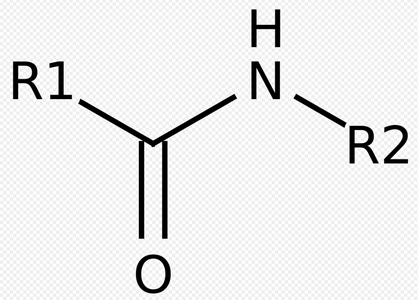
\includegraphics[scale = 0.5]{liaison_peptidique.png} &
   			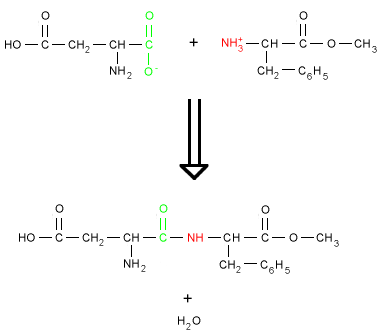
\includegraphics[scale = 0.9]{formation_peptidique.png}\\
		\end{tabular}
		\caption{Gauche : forme générale d'un acide $\alpha-$aminé. Droite : la glycine est le plus 			simple d'entre eux, représentée ici sous forme de zwitterion.}
		\end{center}
	\end{figure}
	
	\item \textbf{Structure des protéines :} quatre niveaux d'organisation
	\begin{itemize}
		\item \textbf{Structure primaire} : séquence en acides aminés;
		\item \textbf{Structure secondaire} : arrangement locaux des acides aminés, 								\textbf{stabilisées par des liaisons hydrogène}, hélices $\alpha$ et feuillets $\beta$;
		\item \textbf{Structure tertiaire} : forme générale de la protéine observable à l'échelle de 				la molécule tout entière (repliement d'une protéine);
		\item \textbf{Structure quaternaire} : complexe résultant de l'assemblage de plusieurs 						molécules de protéines (plusieurs chaînes polypeptidiques), appelées dans ce cas sous-					unités protéiques, pour former un complexe protéique unique. Toutes les protéines ne sont 			pas nécessairement constituées de plusieurs sous-unités et ne possèdent par conséquent 					pas toujours de structure quaternaire.
	\end{itemize}
\end{itemize}

\subsubsection*{Glucose}
\begin{figure}[h!]
	\begin{center}
  		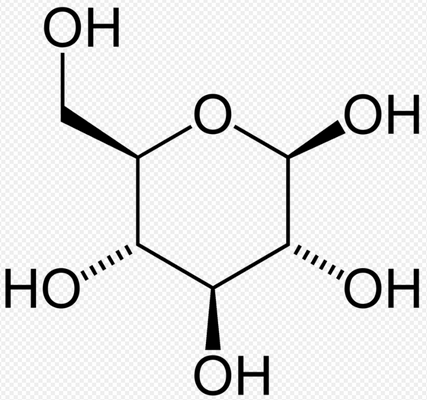
\includegraphics[scale = 0.4]{glucose.png}
	\caption{Glucose.}
	\end{center}
\end{figure}

\end{document}